\hypertarget{rfid_thread_8h}{
\section{RFID\_\-Reader/rfidThread.h File Reference}
\label{rfid_thread_8h}\index{RFID\_\-Reader/rfidThread.h@{RFID\_\-Reader/rfidThread.h}}
}
Erstellt einen Thread, welcher alle 0.5 Sekunden prüft ob eine Karte im Feld des Lesers erscheint. 

{\tt \#include \char`\"{}RFID\_\-CR500.h\char`\"{}}\par
{\tt \#include $<$QtGui$>$}\par


Include dependency graph for rfidThread.h:\nopagebreak
\begin{figure}[H]
\begin{center}
\leavevmode
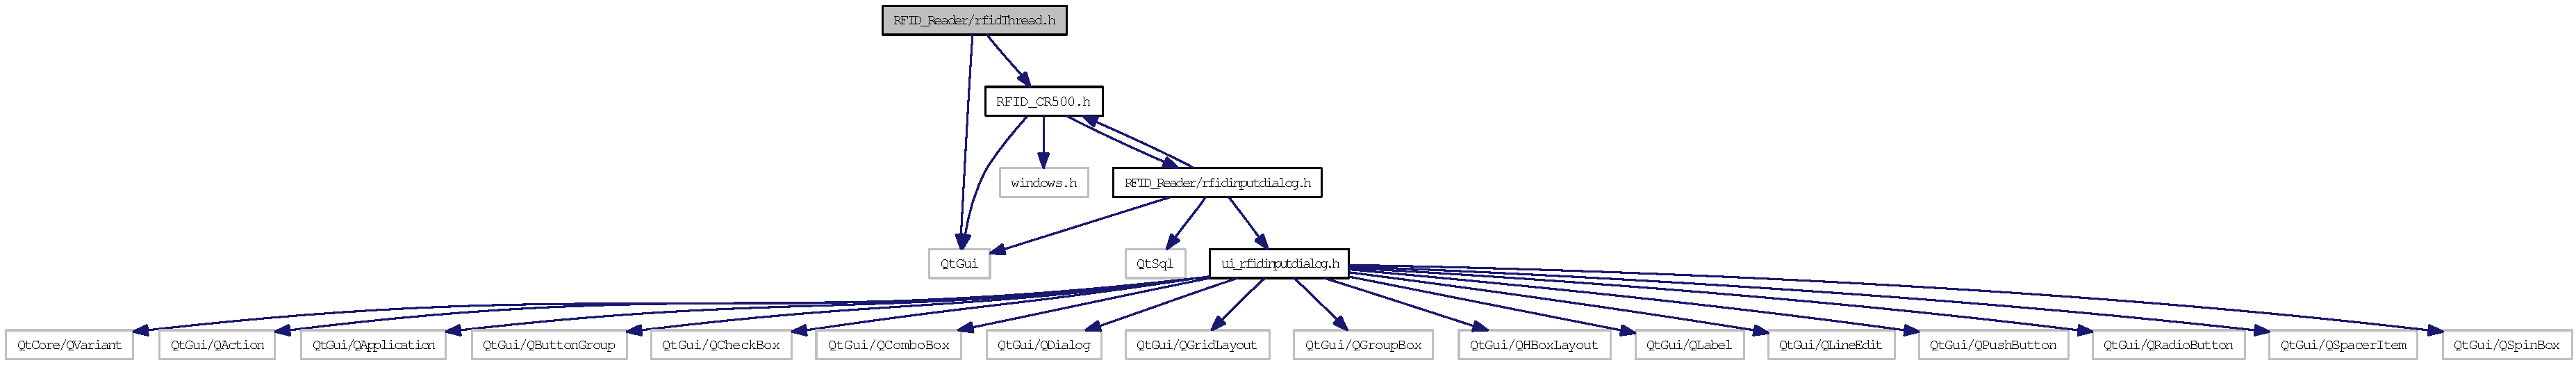
\includegraphics[width=420pt]{rfid_thread_8h__incl}
\end{center}
\end{figure}


This graph shows which files directly or indirectly include this file:\nopagebreak
\begin{figure}[H]
\begin{center}
\leavevmode
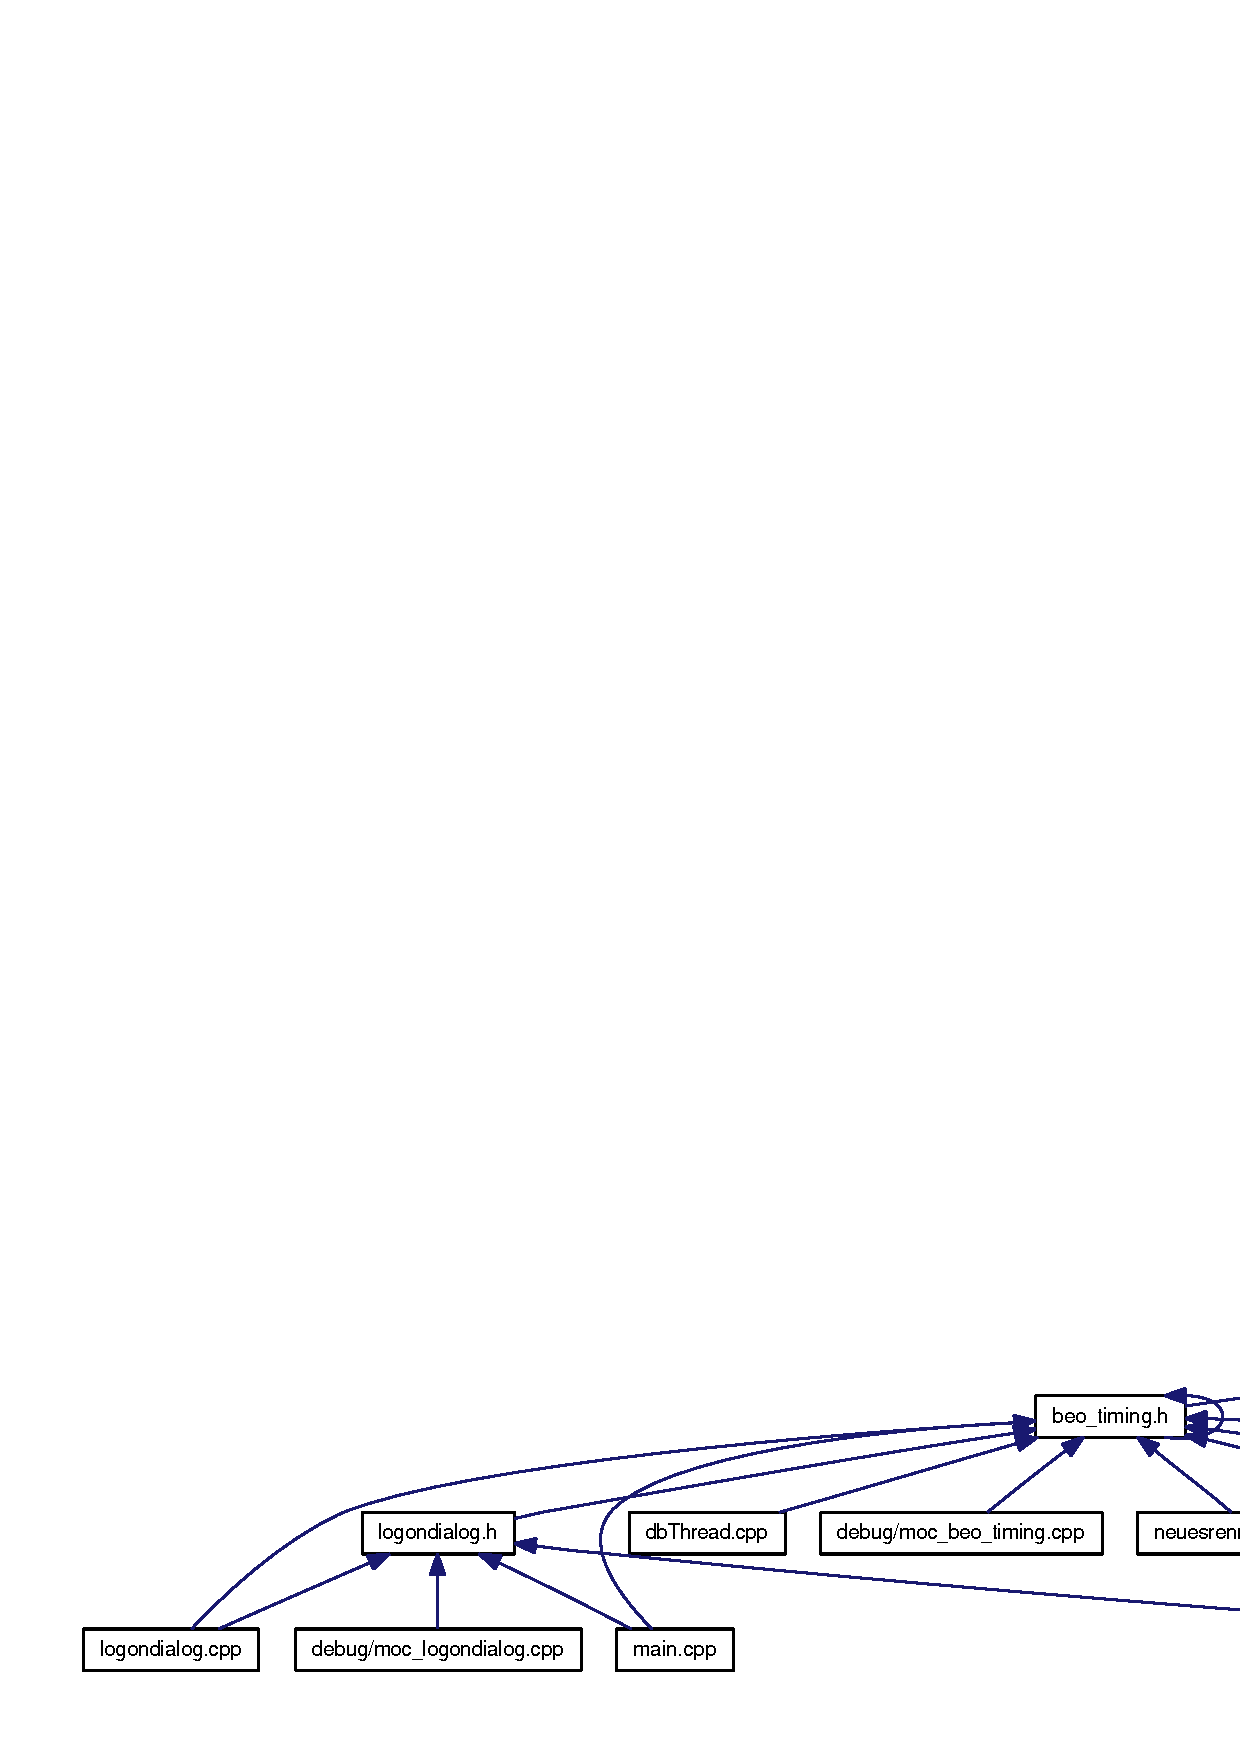
\includegraphics[width=420pt]{rfid_thread_8h__dep__incl}
\end{center}
\end{figure}
\subsection*{Classes}
\begin{CompactItemize}
\item 
class \hyperlink{class_r_f_i_d___thread}{RFID\_\-Thread}
\begin{CompactList}\small\item\em Erstellt einen Thread, welcher alle 0.5 Sekunden prüft ob eine Karte im Feld des Lesers erscheint. \item\end{CompactList}\end{CompactItemize}
\subsection*{Defines}
\begin{CompactItemize}
\item 
\#define \hyperlink{rfid_thread_8h_be5f25a9946157c0aef50f891ae0c4f9}{RFID\_\-REFRESH\_\-RATE\_\-ms}~500
\end{CompactItemize}


\subsection{Detailed Description}
Erstellt einen Thread, welcher alle 0.5 Sekunden prüft ob eine Karte im Feld des Lesers erscheint. 

\begin{Desc}
\item[Version:]1.0 \end{Desc}
\begin{Desc}
\item[Date:]09.06.2008 \end{Desc}
\begin{Desc}
\item[Author:]R.Zoss\end{Desc}
Copyright (C) 2008 Rico Zoss

This file is part of BEO-Timing Managementsoftware.

BEO-Timing Managementsoftware is free software: you can redistribute it and/or modify it under the terms of the GNU General Public License as published by the Free Software Foundation, either version 3 of the License, or (at your option) any later version.

BEO-Timing Managementsoftware is distributed in the hope that it will be useful, but WITHOUT ANY WARRANTY; without even the implied warranty of MERCHANTABILITY or FITNESS FOR A PARTICULAR PURPOSE. See the GNU General Public License for more details.

You should have received a copy of the GNU General Public License along with BEO-Timing Managementsoftware. If not, see $<$\href{http://www.gnu.org/licenses/}{\tt http://www.gnu.org/licenses/}$>$. 

Definition in file \hyperlink{rfid_thread_8h-source}{rfidThread.h}.

\subsection{Define Documentation}
\hypertarget{rfid_thread_8h_be5f25a9946157c0aef50f891ae0c4f9}{
\index{rfidThread.h@{rfidThread.h}!RFID\_\-REFRESH\_\-RATE\_\-ms@{RFID\_\-REFRESH\_\-RATE\_\-ms}}
\index{RFID\_\-REFRESH\_\-RATE\_\-ms@{RFID\_\-REFRESH\_\-RATE\_\-ms}!rfidThread.h@{rfidThread.h}}
\subsubsection[RFID\_\-REFRESH\_\-RATE\_\-ms]{\setlength{\rightskip}{0pt plus 5cm}\#define RFID\_\-REFRESH\_\-RATE\_\-ms~500}}
\label{rfid_thread_8h_be5f25a9946157c0aef50f891ae0c4f9}




Definition at line 38 of file rfidThread.h.

Referenced by RFID\_\-Thread::run().